\documentclass[a4paper,12pt]{article}
\usepackage{graphicx}
\usepackage{hyperref}   % use for hypertext links, including those to external documents and URLs

\begin{document}



\begin{center}
\begin{Huge}
\textbf{{\LARGE Individual Report \\ Unit Test Visualisation Project }}
\linebreak
\linebreak
\linebreak
\linebreak
\end{Huge}\end{center}




\begin{small}
\begin{flushleft}
\textbf{Author:} Sello Ralethe
\\
\textbf{Student Number:} 0708410k
\\
\textbf{Team:} Group 4
\\
\textbf{Course:} ELEN7046 - Software Technologies and Techniques
\\
\textbf{Date Submitted:} 25 June 2012
\\
\textbf{Source \& Documentation:} https://github.com/KeaganPhillips/Wit-Group-4-project
\linebreak
\linebreak
\linebreak
\linebreak
\linebreak
\end{flushleft}

\end{small}


\begin{flushleft}
\textbf{{\large Abstract}}
\end{flushleft}
This paper presents a discussion on the individual work down as a contribution to the group project. The area worked on is given in details, and the methodology, discussing how the work was carried out, is provided. There's also a discussion on the technologies used for implementation. The technologies used are CoffeeScript, HTML5 and KineticJS. This discussion on technologies entails the decisions regarding the selection of certain technologies over others.    
\clearpage


\tableofcontents


\clearpage

\section{Introduction}
One major part of the application developed by my group is the rendering of class diagrams. This is the area that I worked on. The aim of this report is to provide a clear explanation of the role I played in the group, with a discussion on the specific area that I was responsible for. \\

\indent In this report, I will analyse the part of the project that I implemented, and provide an analysis on the area I worked on. I will also provide a discussion on some key design decisions that I had to make. The discussion on design decision is followed by a section discussing the issues encountered during coding.\\

\indent The design decisions I made influence the choice of technologies I used for the implementation. Also, the overall design of the system played an important part. The technologies I used are coffee script and html5. Specifically, I utilised KineticJS, which is an HTML5 canvass JavaScript library
The remainder of this report is as follows. Section 2 discusses the area that I worked on in depth, and in a way formulate the problem to be solved. The approach to the solution is given in section 3. I then discuss the technologies used to solve the problem in section 4. How these technologies were applied in the solution is provided in section 5. 

\section{Individual Contribution}
The developed application displays all the classes under test on the canvas. The classes displayed are not static, and can be dragged within the canvas in which they are displayed. Clicking on a class is shown by highlighting that class with a different colour from other classes.\\

\indent The following picture shows how a selected class looks like: 
\begin{figure} [H]
\includegraphics[scale=0.8] {capture.png}
\caption{A selected Class Diagram}
\label{mdp}
\end{figure}

To accomplish this, I had to undertake several tasks. These are:
\begin{itemize}
\item Read in data generated by the backend application
\item Loop through the data, extracting the class name, public methods and public properties.
\item Draw classes from this extracted data
\item Ensure that the classes are moveable and selectable.
\end{itemize}
The data from the backend comes through a JSON data structure. Figure 2 is an example that shows the JSON representation of an object that describes a class
\indent The following picture shows how a selected class looks like: 
\begin{figure} [H]
\includegraphics[scale=0.8] {capture1.png}
\caption{JSON Data Structure}
\label{mdp}
\end{figure}

\indent My role involved iterating through the data, and displaying it in the form of classes with methods and properties. Because the number of classes in the data could only be determined at runtime, this influenced the choice of the programming language. One feature of the chosen technology for implementation was that it caters for the creation of classes and objects. So drawing class diagrams was accomplished by utilising a single class to automate the drawing of the class diagrams on the canvas. Figure 3 shows the overview of the tasks in the overall system that I worked on.
\indent The following picture shows how a selected class looks like: 
\begin{figure} [H]
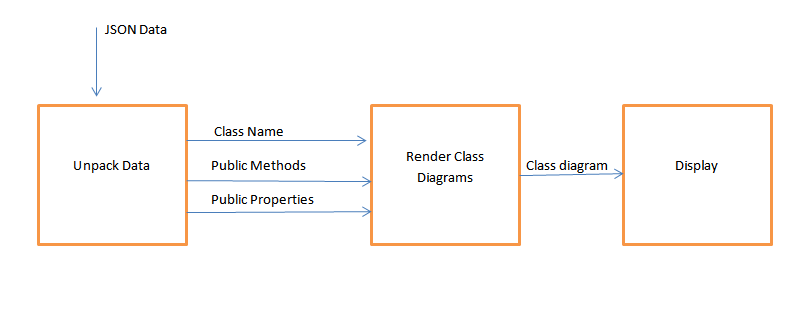
\includegraphics[scale=0.8] {design.png}
\caption{A selected Class Diagram}
\label{mdp}
\end{figure}


\section{Methodologies and Approach}
To carry out the tasks I set up a plan, with deadlines on it. The initial task was to learn CoffeeScript as I had no experience with it. Initially I gave myself 16 hours spread over 3 days to learn CoffeeScript. During the learning process, I realised that I needed to brush up on some features of JavaScript because debugging CoffeeScript is, in essence, debugging JavaScript. This minor setback required adding another day to the initial plan, and in a way delaying the plan by a day. \\

\indent The next step after CoffeeScript was to familiarise myself with the JavaScript Object Notation (JSON). This is a lightweight data-interchange format. My initial estimate for the duration of this task was higher than the time I spent on it. I think the reason I spent less time on JSON was that I was familiar with JavaScript, so this helped to speed up the learning. From this occurrence, my progress was ahead of schedule.\\

\indent I used the extra time gained from the previous task to start looking at implementation. The realisation was that although my design of rendering class diagrams could be implemented in any scripting language, CoffeeScript was the favourite language of choice due to the fact that it can be implemented in classes, unlike JavaScript.\\

\indent The next task was to read the JSON data, extract information from it and then display this information. Since this was the major task of all the tasks, I planned to spend a lot of time on it. This task required knowledge in HTML5 canvas. Learning how to work in HTML5 took less time, since I knew which aspect of HTML5 I needed to know in order to carry out the task. \\

\indent After displaying the classes, the next task was to enable the user to be able to move the classes around. This feature was implemented using HTML5. The use of HTML5 ensured that there is no need to have a plugin that enables the movements on the browser. So utilising HTML5 was a good choice of technology. 
The last task in my list of tasks required collaboration with one of my group members. This was because an event caused by the part of the application I developed triggers an event in the other part of the application developed by Demi. When the user clicks on a class diagram, some information is sent to the part of the application that Demi worked on. \\

\indent Besides having to collaborate with Demi, I had to design how the click event works, and how the user would see that he/she has clicked on a certain class. To do this, I simply had to highlight the boarders of the class clicked.\\

\indent Even though I had a minor setback in the beginning of my plan, I managed to deliver my part of the program in time for the integration with modules developed by the rest of the team. Appendix B highlights the actual plan I followed to carry out my tasks.

\section{Technologies Utilised}
This section discusses the technologies that I used for implementation. The discussion is merely a high-level overview of the technologies.
\subsection{CoffeeScript}
CoffeeScript is a language that compiles into JavaScript. It brings new elegance and efficiency to the writing of JavaScript. It does this by helpfully enforcing JavaScript best practices. Briefly explained, CoffeeScript is a thin syntactical layer on top of JavaScript. CoffeeScript shares most of the same constructs with JavaScript, but with a different, tighter syntax.\\

\indent It has been widely realised in the last few years that JavaScript is a most excellent language when wielded right, utilising its expressiveness and applying functional programming.
CoffeeScript aims to negate the clunky syntax of JavaScript. By sacrificing the ability to have many statements on a single line, CoffeeScript negate the need for semicolons completely. CoffeeScript also strives to be more readable, by changing existing keywords and operators to more succinct and self-explanatory versions. Thus the keyword "function" is distilled down to the simple dash rocket$ "->"$, equality is {"is"} instead of {"=="}, and so forth.\\

\indent CoffeeScript adds new keywords to simplify commonly occurring patterns. This includes class declaration, prototype access, destructuring assignments, loops, and many more. These concepts are a very powerful way of shortening code. This is also the reason CoffeeScript is almost always half or less of the size of the generated JavaScript.\\

\indent One of the aims in creating CoffeeScript was for there to always be a 1-to-1 correspondence with JavaScript. This makes it easy for someone already into JavaScript to adopt CoffeeScript and sharpen their skills. It also means that CoffeeScript can be used with any and all JavaScript library.\\

\indent There are some features of JavaScript that are made better and simpler in CoffeeScript. One of these features is how iteration over arrays works. The great thing about this is that it works together with jQuery. Another feature allows for the binding of methods on the fly. Using this feature inside of a jQuery call-back saves the hassle of manually binding methods to objects. With CoffeeScript, one can easily distribute arguments of methods with long signatures such as ".post()" and ".animate()" over multiple lines. Commas and curly brackets are optional. This adds to the readability of many of jQuery's method calls.\\

\indent With all its nice features, CoffeeScript has some drawbacks. One notable drawback is that CoffeeScript introduces a new step in the build process, as the code has to be compiled to JavaScript before it is used. This is trivial once a setup is made to auto-compile whenever the CoffeeScript file is saved. However, that initial setup still has to be done.\\

\indent Another drawback is with regard to debugging. For runtime errors, CoffeeScript returns line numbers referencing the generated JavaScript code instead of the original CoffeeScript file. What I experienced was that if you know where in the CoffeeScript code the bud is, then debugging is fairly easy. If this is not the case, then debugging becomes a difficult task: you have to open the generated file, find the line, deduce from the context what CoffeeScript function this correlates to, then find that corresponding section in the CoffeeScript file and fix the error.\\

\indent Whether the pros outweigh the cons is of course heavily situational, depending both on the individuals and the project. A performance gain of CoffeeScript over JavaScript can come from optimising features. For example, CoffeeScript stores the array length in a separate variable in a for-loop instead of requesting it in every iteration. 


\subsection{HTML5}
HTML5 is the fifth major revision of HTML. Unlike older versions of HTML, this new one is designed to do more things. For instance, animations can be displayed directly in the browser without a plugin.
I utilised HTML5 canvas to draw graphics and to implement motions and click events. A canvas is a drawable region defined in HTML code with height and width attributes. Canvas has several methods for drawing paths, boxes, circles, characters, and adding images.\\

\indent HTML5 canvas allows for the drawing of graphics on the fly using a scripting language such as CoffeeScript or JavaScript. To draw graphics on the canvas, I utilised KineticJS, which is an HTML5 JavaScript library.\\

\indent With the capability of "high performance path detection", KineticJS runs fast and can work with thousands of shapes at the time. With KineticJS, I can draw my own shapes using the existing canvas API, add event listeners to them, move them, scale them, layer them on top of each other, and rotate them independently from other shapes. \\

\indent Most important feature of KineticJS is that it enables using every object like a layer. HTML5 canvas doesn’t have this feature by default. Also, the stacks feature helps grouping layers to control them better. For instance, I created a box as a layer, then added text to that layer, and then set the layer to be moveable so that by dragging the layer, the text also moves along with the motion of the box.
KineticJS applications require a container Document Object Model (DOM) element in the HTML page to contain a stage which is made up of layers. The DOM is the way JavaScript sees its containing pages’ data. It is an object that includes how HTML is formatted, as well as the browser state. Classes can be added to DOM using JavaScript. In my case I used CoffeeScript. Under KineticJS, each layer created is tied to its own canvas element, and can contain groups or shapes.\\

\indent For event handling, the KineticJS stage is made up of a backstage layer and a buffer layer, together with event detection throttling to prevent excess event detections. The backstage layer is a hidden layer that uses a custom canvas context to render invisible shapes. The buffer layer is also a hidden layer that is used for pixel detection and canvas composites. Features such as animations, transitions, and drag and drop operations are particularly smooth because developers can create an unlimited number of user defined layers which enable them to update and redraw some shapes while not touching others.\\

\indent These features enabled me to do the following. Firstly, I drew empty boxes during runtime. The dimensions of the boxes were determined by how long the texts are. For instance, the length of a class name determined the width of the box, while the number of properties plus methods determined the height of the box. Once the boxes where drawn, I added texts on the layer containing the boxes and then set drag and drop properties of the layer to be true. This enabled the boxes to be moved around the screen independent of each other.


\section{Conclusion}
In this paper, I presented the area that I worked on for the group project. I was responsible for rendering class diagrams and displaying them in the browser. I had a plan on how I was going to deliver the task assigned to me. I followed the plan, with only one minor setback. However, that setback did not delay my progress. The decision of overestimating the sizes of tasks lead to me finishing them ahead of time, and within schedule. \\

\indent I had choices regarding which technologies to use for implementing my design. From the technologies at my disposal, I chose one that complemented the design. Due to time being a factor and the limited skills I possess, I could not experiment with other technologies.\\

\indent The part that I worked on was implemented using scripting languages. Working with CoffeeScript enabled me to work with classes. Unlike JavaScript, CoffeeScript allows for the creating of objects using classes. Objects in JavaScript are not created using classes. This is because JavaScript does not support class-based inheritance.\\

\indent By working on this part of the project, I had the opportunity to learn new skills. This includes learning CoffeeScript, KineticJS and HTML5 canvas.

 


\end{document}